\documentclass[a4paper]{usiinfbachelorproject}

\captionsetup{labelfont={bf}}
\usepackage{float}
\usepackage{amsmath}
\usepackage{graphicx}
\usepackage{enumitem}
\usepackage{booktabs}
\usepackage{hyperref}

\author{POLAD BAKHISHZADE}

\title{\textbf{LLM as Code-Correctness Judge}}
\subtitle{Unveiling the Causes of Large-Language-Model Failures when Assessing Java Code}
\versiondate{\today}

\begin{committee}
  \advisor[Università della Svizzera italiana, Switzerland]{ }{Gabriele}{Bavota}
  \coadvisor[Università della Svizzera italiana, Switzerland]{ }{Giuseppe}{Crupi}
\end{committee}

% ——————————————————————————— ABSTRACT
\abstract{
\textbf{Context.}  
Large Language Models (LLMs) are increasingly being used in software development tasks such as code generation, explanation, and bug fixing. An emerging frontier is the use of LLMs for code review—specifically, assessing whether a given implementation is functionally correct. This requires reasoning over both the specification and the code, making it a strong benchmark for code understanding.\\
\\[2pt]
\textbf{Objective.}  
This study investigates how the quality and quantity of natural-language context affect the ability of LLMs to assess code correctness. We ask: \emph{What kind of descriptive information helps or harms the model’s ability to judge whether a function is correct?}\\
\\[2pt]
\textbf{Method.}  
We extend the Java subset of the \textsc{CoderEval} benchmark by systematically enriching it with five structured documentation layers—ranging from brief summaries to formal pre/post-conditions. Each of 362 functions is paired with one correct and one incorrect candidate implementation. We then prompt three open LLMs—Qwen-0.5B, Qwen-1.5B, and DeepSeek-1.3B—to act as zero-shot code judges, under multiple prompt configurations.\\
\\[2pt]
\textbf{Findings.}  
The results reveal that different models respond differently to added context: smaller models benefit from concise behavioral descriptions but often degrade when presented with verbose examples or formal constraints. In contrast, larger models leverage detailed descriptions to reduce mistakes and achieve more reliable judgments. Some layers, such as examples, can introduce confusion and accuracy drop depending on the model.\\
\\[2pt]
\textbf{Outcome.}  
The study highlights the importance of model-specific prompt design and shows that more documentation is not always better. These insights can inform future systems that rely on LLMs for code quality assessment.\\
\\[2pt]
\textbf{Keywords}: LLMs; Code Review; Code Correctness; Prompt Engineering; Evaluation; Java; Dataset Enrichment
}

\begin{document}
\maketitle
\tableofcontents\newpage

% ——————————————————————————— 1 INTRODUCTION
\section{Introduction}\label{sec:intro}
Large Language Models (LLMs) such as ChatGPT, GitHub Copilot, and StarCoder have become widely adopted in software development workflows. Originally developed for general language understanding, these models have rapidly gained traction in code-related tasks, including code generation, explanation, repair, and synthesis. Researchers are increasingly exploring the use of LLMs for more advanced code understanding tasks, such as debugging, static analysis, and functional correctness evaluation.\\
\\[2pt]
Among the many challenges in this space, one particularly important question is whether LLMs can serve as reliable evaluators of automatically generated code. In industrial settings, such as at Google, the proportion of code written or assisted by machine learning systems is steadily increasing. However, verifying the correctness of such code remains an open problem. Traditional techniques like writing unit tests are time-consuming and require substantial human effort, creating a bottleneck in workflows that rely heavily on automated code generation. This motivates the need for automatic, oracle-free evaluation mechanisms capable of assessing whether a candidate implementation adheres to a given specification.\\
\\[2pt]
Despite promising results in code generation, LLMs’ reliability in evaluating correctness remains underexplored. Much of the existing work focuses on generation benchmarks with minimal or vague natural language descriptions, which offer limited insight into how models reason about correctness. Furthermore, it is unclear how the structure and depth of the task description impact the model’s evaluation ability.\\
\\[2pt]
In this work, we investigate whether more detailed and structured descriptions help LLMs better judge the correctness of candidate implementations. Specifically, we extend the \textsc{CoderEval} benchmark by enriching each function with five levels of natural language documentation, ranging from a one-line summary to detailed behavioral, signature-level, example-based, and pre/postcondition specifications. We evaluate three instruction-tuned models—Qwen-0.5B, Qwen-1.5B, and DeepSeek-1.3B—across 362 function–candidate pairs, comparing their accuracy under cumulative and ablation prompt settings.\\
\\[2pt]
Our results suggest that model capacity plays a significant role in how different types of documentation are utilized. Smaller models, such as Qwen-0.5B, benefit from concise behavioral context but are negatively impacted by verbose or redundant input. In contrast, Qwen-1.5B leverages detailed structure effectively, showing consistent accuracy gains as more layers are added. Meanwhile, DeepSeek-1.3B performs best with minimal input and degrades when faced with richer prompts—suggesting sensitivity to verbosity and limited ability to exploit complex descriptions. These findings highlight the importance of prompt design in aligning LLM reasoning with software correctness.

\subsection*{Report structure}

Section~\ref{sec:related} reviews related literature.  
Section~\ref{sec:design} presents our study design and dataset enrichment pipeline.  
Section~\ref{sec:results} covers results from cumulative and ablation experiments.  
Section~\ref{sec:concl} concludes and outlines future directions.

% ——————————————————————————— 2 RELATED WORK
\section{Related Work}\label{sec:related}

The use of Large Language Models (LLMs) for code understanding and evaluation has become an active area of research. While LLMs have demonstrated impressive capabilities in code generation tasks, recent work highlights a critical gap in their ability to evaluate or judge the correctness of code—a task that requires genuine semantic understanding rather than pattern memorization.\\
\\[2pt]
Several studies have investigated this limitation. West et al.~\cite{west2023generative} introduce the "Generative AI Paradox", noting that models often produce high-quality outputs without fully understanding them. Gu et al.~\cite{gu2024counterfeit} further expose this gap through the "Counterfeit Conundrum", showing that LLMs struggle to recognize subtle flaws in their own generations. These findings suggest that correctness judgment is a non-trivial challenge, especially in the absence of explicit oracles such as test cases.\\
\\[2pt]
In response to this, researchers have proposed new benchmarks and evaluation strategies. Zhao et al.~\cite{zhao2024codejudgeeval} present CodeJudge-Eval, a benchmark specifically designed to test whether LLMs can distinguish correct from incorrect implementations. The results reveal that even strong models frequently misclassify buggy or misleading solutions, reinforcing that functional correctness evaluation remains an open question. Similarly, Zhuo~\cite{zhuo2023icescore} introduces ICE-Score, an instruction-based metric where LLMs are explicitly guided to assess code correctness and quality. This approach avoids traditional test-based evaluation and aligns with the growing interest in oracle-free evaluation pipelines.\\
\\[2pt]
Building on ICE-Score, Tong and Zhang~\cite{tong2024codejudge} propose CodeJudge, a more structured framework where LLMs are prompted to follow a multi-step "slow thinking" process before rendering a correctness decision. Their results demonstrate that structured prompting can significantly improve evaluation quality, even when using relatively small models. Our study builds on these insights by also employing layered prompt structures but focuses more explicitly on how the level of detail and structure in descriptions interacts with model capacity.\\
\\[2pt]
Other efforts have focused on aligning LLM judgments with human preferences or pedagogical goals. Weyssow et al.~\cite{weyssow2024codeultrafeedback} introduce CodeUltraFeedback, a dataset where 14 LLMs respond to coding instructions and are judged on dimensions such as readability, style, and instruction-following. Their findings suggest that LLMs can be aligned to human-like evaluation standards through supervised fine-tuning. While our work also investigates LLMs-as-judges, our focus is on functional correctness rather than stylistic alignment.\\
\\[2pt]
The educational domain provides additional context. Koutcheme et al.~\cite{koutcheme2025evaluating} explore whether LLMs can generate and assess programming feedback in student assignments. Their findings suggest that LLMs—both open-source and proprietary—are approaching the reliability of human graders in introductory programming contexts. Though focused on feedback generation rather than correctness verification, this line of work highlights the growing confidence in LLM-based evaluation systems.\\
\\[2pt]
In summary, prior work has identified the limits of current LLMs in judging code, proposed structured prompting techniques and evaluation metrics, and explored domain-specific use cases. Our study complements these directions by incrementally enriching the prompt descriptions and examining how different model sizes respond to varying levels of contextual detail when judging code correctness.


% ——————————————————————————— 3 STUDY DESIGN
\section{Study Design}\label{sec:design}

\subsection*{Research question}
\noindent\textbf{RQ} –  
\emph{To what extent the information reported in the code description impact the ability of the LLMs to judge the correctness of a given code?}

\subsection{Models evaluated}\label{sec:models}
\begin{itemize}[leftmargin=12pt,itemsep=1pt]
  \item \textbf{Qwen-0.5B Instruct} (0.5 B params).  
  \item \textbf{Qwen-1.5B Instruct} (1.5 B).  
  \item \textbf{DeepSeek-Coder-1.3B Instruct}.  
\end{itemize}

\subsection{Dataset}\label{sec:dataset}
From the Java subset of \textsc{CoderEval}:
\begin{enumerate}[label=\alph*),leftmargin=14pt,itemsep=0pt]
  \item Removed noisy IDs.  
  \item For each remaining ID, selected one correct and one incorrect candidate (existing model outputs).  
\end{enumerate}
Final size: \textbf{362} rows (balanced).

\subsection{Documentation layers}\label{sec:layers}
\begin{description}[style=nextline,leftmargin=15pt]
  \item[L1] Summary (1 sentence).  
  \item[L2] Behaviour narrative (detailed summary).  
  \item[L3] Signature description (argument/return semantics).  
  \item[L4] Examples (I/O pairs).  
  \item[L5] Pre/post-conditions.  
\end{description}
ChatGPT-4o generated all layers for each of 181 Java functions.

\subsection{Prompt template}
\textbf{Constant preamble}: task, label scheme (`0/1`, no extra text).\\
\textbf{Variable payload}: selected layers + \textit{first line of candidate code} (argument/return).\\
\textbf{Generation}: temperature 0.2, max\_new\_tokens 20.

\subsection{Experimental conditions}
\textbf{Incremental} (5 runs):
\[
\text{L1};\; \text{L1+L2};\; \text{L1+L2+L3};\; \text{L1+L2+L3+L4};\; \text{L1+L2+L3+L4+L5}
\]
\textbf{Ablations}:
\[
\text{No L1};\; \text{No L2};\; \text{No L4};\; \text{No L5}
\]

\subsection{Metrics}
TP, TN, FP, FN; Accuracy = (TP+TN)/362.

\subsection{Project Repository}
\href{https://github.com/poladbachs/Bachelor-Thesis}{\texttt{github.com/poladbachs/Bachelor-Thesis}}.

% ——————————————————————————— 4 RESULTS
\section{Results \& Discussion}\label{sec:results}

%------------------------------------------------------------------
\subsection{Incremental enrichment (L1 $\rightarrow$ L5)}
%------------------------------------------------------------------

\begin{figure}[H]\centering
  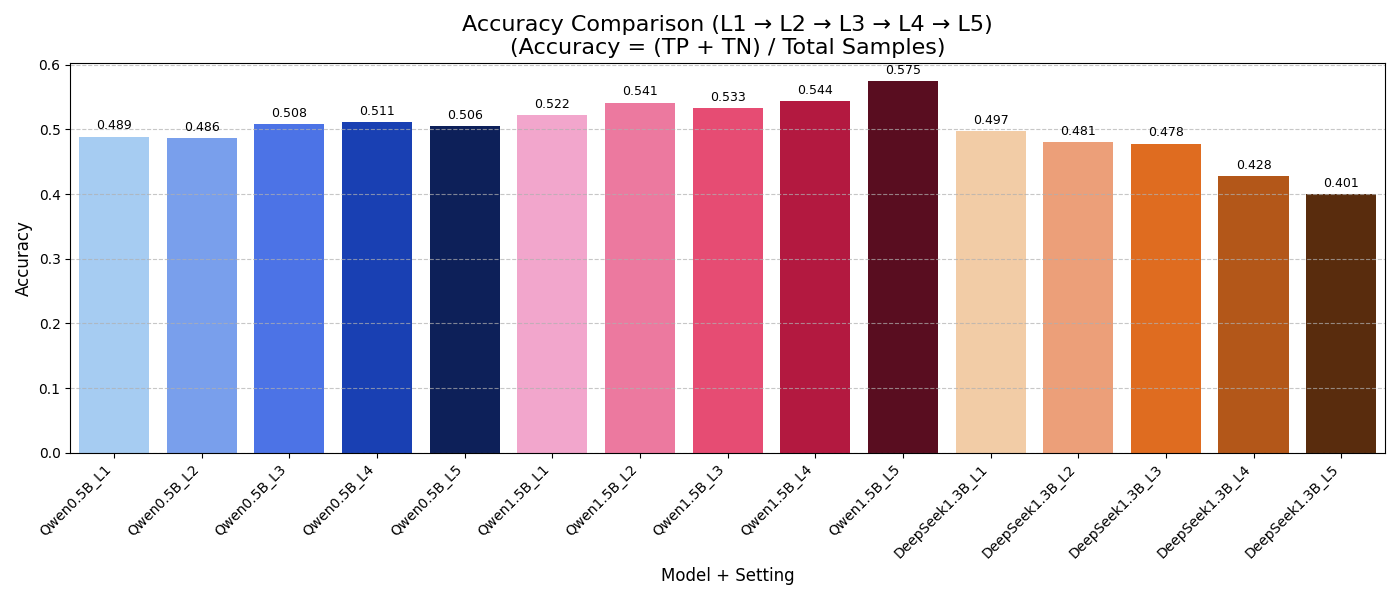
\includegraphics[width=0.95\linewidth]{figures/accuracy_comparison.png}
  \caption{Accuracy per model and documentation level.}
  \label{fig:acc-l1-l5}
\end{figure}

\paragraph*{Accuracy trends.}
We observe clear divergence in how each model responds to additional natural-language context:

\begin{itemize}[leftmargin=12pt]
  \item \textbf{Qwen-0.5B}: After stagnating on L1–L2, the model improves through L3 and L4, peaking at 0.511. L5 slightly degrades performance, suggesting diminishing returns or confusion from formal logic.
  
  \item \textbf{Qwen-1.5B}: Displays consistent benefit from each additional layer, rising steadily to 0.575 at L5. This model appears to handle verbosity well and leverages the full specification.

  \item \textbf{DeepSeek-1.3B}: Begins strong at 0.497 with minimal input, but drops with every added level—falling below 0.41 at L5. More context leads to worse performance, implying overload or poor instruction tuning for interpretive tasks.
\end{itemize}

These trends support our core hypothesis: smaller models benefit from concise cues, while larger models thrive on richer context. However, more detail is not universally helpful—its usefulness depends on model capacity and internal robustness to verbosity.

\vspace{0.8em}

% --------------------------- Qwen-0.5B
\begin{figure}[H]\centering
  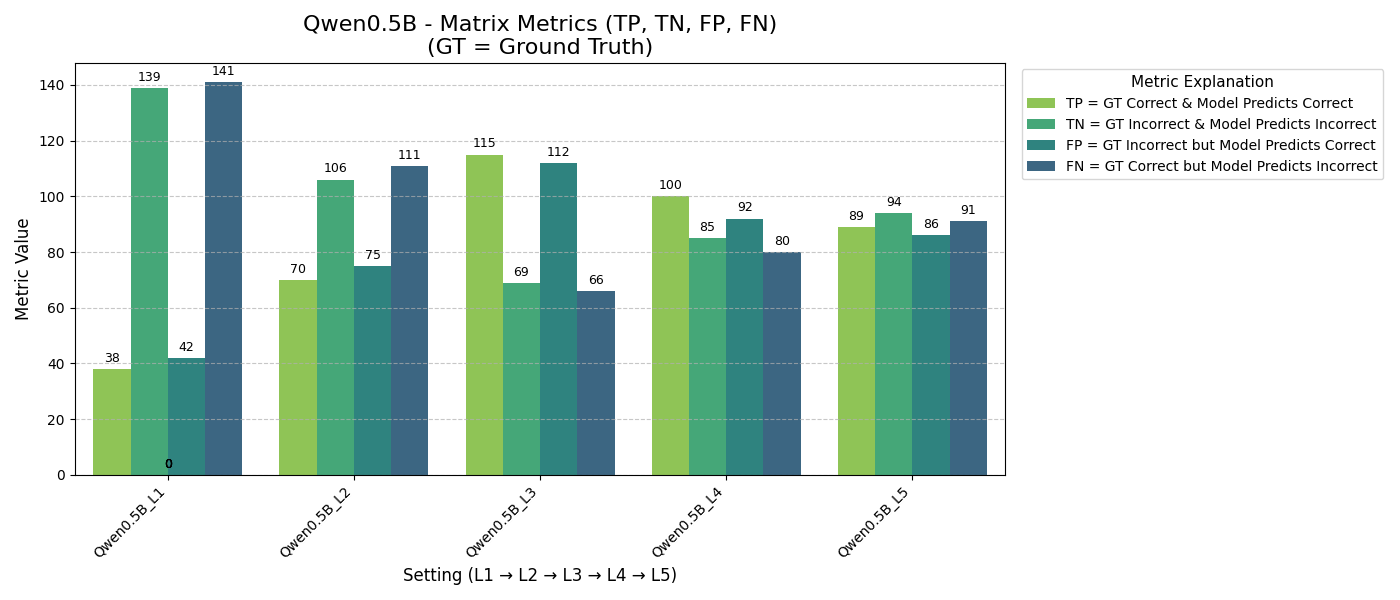
\includegraphics[width=\linewidth]{figures/Qwen0.5B_matrix_metrics.png}
  \caption{Confusion-matrix metrics — Qwen-0.5B.}
  \label{fig:q05-matrix}
\end{figure}

\paragraph*{Interpretation — Qwen-0.5B.}
Early stages (L1–L2) show a struggle to distinguish correct from incorrect implementations, with high false negatives. L3 and L4 reduce FN significantly, converting many correct cases into true positives. However, at L5 false positives creep back in, suggesting that formal conditions (pre/post) mislead the model or increase ambiguity. Overall, Qwen-0.5B needs concise clarity—too much structure destabilizes its judgment.

\vspace{0.8em}

% --------------------------- Qwen-1.5B
\begin{figure}[H]\centering
  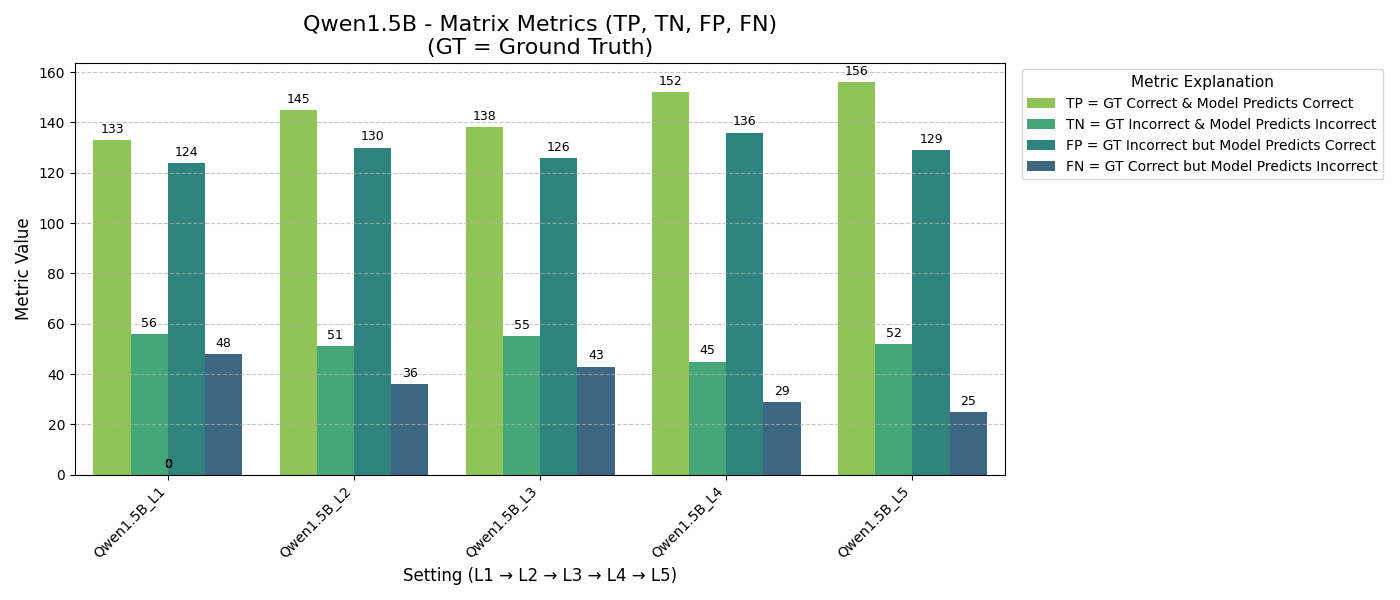
\includegraphics[width=\linewidth]{figures/Qwen1.5B_matrix_metrics.png}
  \caption{Confusion-matrix metrics — Qwen-1.5B.}
  \label{fig:q15-matrix}
\end{figure}

\paragraph*{Interpretation — Qwen-1.5B.}
The larger Qwen model handles incremental context with ease. As layers are added, false negatives drop sharply while true positives grow, especially after L4–L5. Pre/post-conditions help the model rule out wrong implementations without over-predicting correctness (FP stays stable). The balance between increased TP and maintained TN implies that Qwen-1.5B is the most context-aware model among the three.

\vspace{0.8em}

% --------------------------- DeepSeek-1.3B
\begin{figure}[H]\centering
  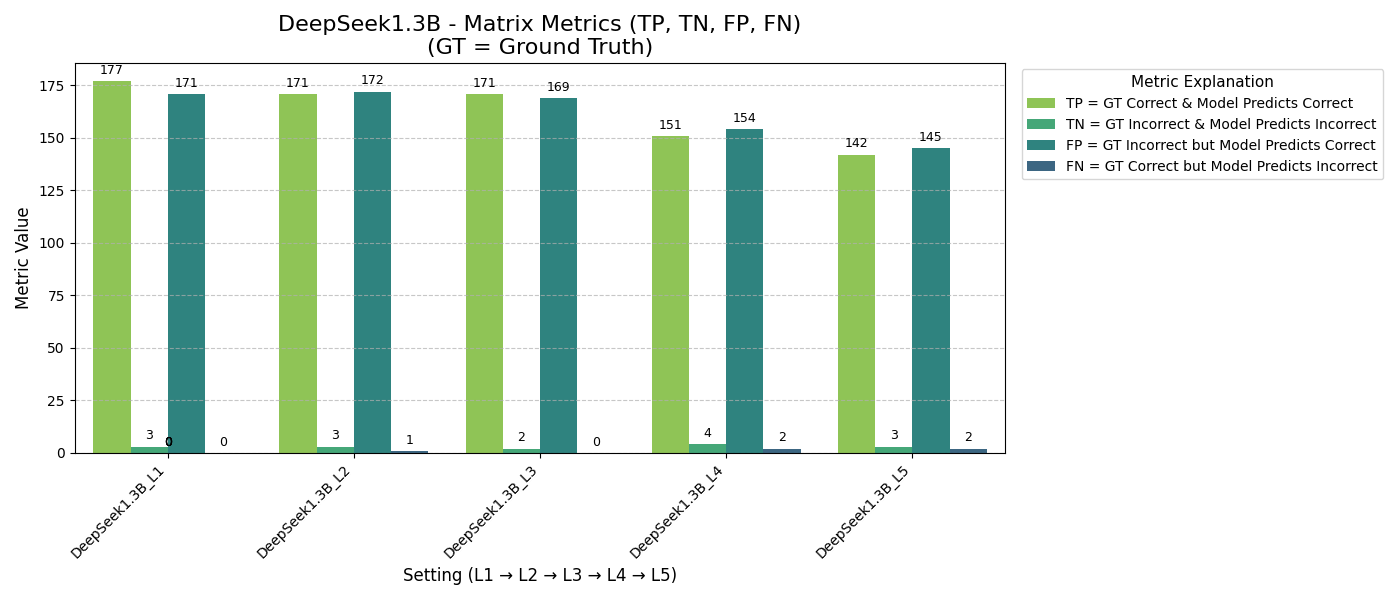
\includegraphics[width=\linewidth]{figures/DeepSeek1.3B_matrix_metrics.png}
  \caption{Confusion-matrix metrics — DeepSeek-1.3B.}
  \label{fig:ds-matrix}
\end{figure}

\paragraph*{Interpretation — DeepSeek-1.3B.}
Despite its comparable size, DeepSeek behaves like a brittle small model in judgment tasks. At L1 and L2, it achieves high TP with minimal FN. But starting at L3, false positives spike and true negatives collapse. This suggests that the added details—examples, constraints—shift attention away from core logic and confuse decision boundaries. It likely overfocuses on surface patterns in examples, falsely validating buggy code.



\subsection{Single-layer ablations}

\begin{table}[H]\centering
\caption{Accuracy after removing one layer. Values in parentheses show the change relative to the full prompt (L1--L5).}
\begin{tabular}{lccc}
\toprule
\textbf{Model} & \textbf{No L1} & \textbf{No L2} & \textbf{No L4} \\ \midrule
Qwen-0.5B  & 0.481 (–0.025) & \textbf{0.450 (–0.056)} & 0.494 (–0.012) \\
Qwen-1.5B  & 0.572 (–0.003) & 0.558 (–0.017) & 0.552 (–0.023) \\
DeepSeek-1.3B & \textbf{0.500 (+0.099)} & 0.434 (+0.034) & 0.428 (+0.028) \\
\bottomrule
\end{tabular}
\end{table}

\paragraph*{Interpretation.}
\begin{itemize}[leftmargin=12pt,itemsep=0pt]
  \item Removing behaviour (L2) cripples Qwen-0.5B (–5.6pp) $A \Rightarrow B$
 small model needs that layer.  
  \item Summary (L1) is useless or noisy for DeepSeek (+9.9pp when removed).  
  \item Qwen-1.5B tolerates all removals ($\leq$2pp), showing robustness.
\end{itemize}

\subsection{Compound ablations (illustrative)}

For space we discuss one illustrative combo per model:

\begin{itemize}[leftmargin=12pt]
  \item \textbf{Qwen-0.5B No L1 \& No L4}: accuracy 0.506 (–0.006 vs. full) — removing summary offsets example noise.  
  \item \textbf{Qwen-1.5B No L1 \& No L4}: 0.558 (–0.017) — examples help this model.  
  \item \textbf{DeepSeek No L2 \& No L4}: 0.478 (+0.078) — minimal prompt is best.  
\end{itemize}

\subsection{What makes a layer “noisy”?}
Manual error analysis highlights three patterns:

\begin{enumerate}[label=\alph*),leftmargin=15pt,itemsep=0pt]
  \item \textbf{Example bias}.  L4 lists only happy-path cases → model over-predicts “correct”.  
  \item \textbf{Narrative redundancy}.  L2 restates corner cases differently from L5, confusing alignment.  
  \item \textbf{Generic summaries}.  L1 adds little entropy; for DeepSeek it seems to trigger a “looks plausible → correct” bias.
\end{enumerate}

% ——————————————————————————— 5 CONCLUSIONS
\section{Conclusions \& Future Work}\label{sec:concl}

\begin{itemize}[leftmargin=12pt]
  \item Moderate enrichment (+behaviour, +signature) boosts small models (+8pp).  
  \item Verbose layers (examples, formal conditions) help mid-size models but harm 0.5 B and DeepSeek.  
  \item Removing noisy layers (summary or examples) can recover performance (DeepSeek +10pp).  
\end{itemize}

\textbf{Next steps}.  
\begin{enumerate}[label=\arabic*.]
  \item Fine-tune a 0.5 B checkpoint on the enriched dataset.  
  \item Auto-select minimal counter-examples to make L4 compact and balanced.  
  \item Extend to Python and larger open models (e.g.\ Llama-3-8B).  
\end{enumerate}

% ——————————————————————————— REFERENCES
\bibliographystyle{abbrv}
\bibliography{references}

\end{document}
